\documentclass[a4paper]{beamer}%handout


\usepackage{listings}
\usepackage{color}
 
\definecolor{codegreen}{rgb}{0,0.6,0}
\definecolor{codegray}{rgb}{0.5,0.5,0.5}
\definecolor{codepurple}{rgb}{0.58,0,0.82}
\definecolor{backcolour}{rgb}{0.95,0.95,0.92}


%% Add Matlab code
\usepackage{mcode}
%% Add Matlab code end


%% Add watermarks
%\usepackage{draftwatermark}
%% Add watermarks end
\usepackage[utf8]{inputenc}
\usepackage{multicol}
\usepackage{url}
\usepackage{hyperref}
\hypersetup{
	colorlinks=true,
	linkcolor=cyan,          % color of internal links (change box color with linkbordercolor)
    citecolor=green,        % color of links to bibliography
    filecolor=magenta,      % color of file links
    urlcolor=cyan           % color of external links
	}

\graphicspath{{img/}}

\mode<presentation> {

%\usetheme{default}%yes % use %\frametitle in all slides recommended
%\usetheme{AnnArbor}%no
%\usetheme{Antibes} %yes %favorite
%\usetheme{Bergen} %no
%\usetheme{Berkeley} %no
%\usetheme{Berlin} %no
%\usetheme{Boadilla} %yes % good use of paper space
%\usetheme{CambridgeUS} %yes %favorite %use %\frametitle recommended
%\usetheme{Copenhagen}%yes%noframetitle
%\usetheme{Darmstadt}%no
%\usetheme{Dresden}
%\usetheme{Frankfurt}
%\usetheme{Goettingen}
%\usetheme{Hannover}
%\usetheme{Ilmenau}%no
%\usetheme{JuanLesPins}
%\usetheme{Luebeck}
%\usetheme{Madrid}
%\usetheme{Malmoe}
%\usetheme{Marburg}
%\usetheme{Montpellier}
%\usetheme{PaloAlto}
%\usetheme{Pittsburgh}%no
%\usetheme{Rochester}%no
%\usetheme{Singapore}%yees
%\usetheme{Szeged}%no
%\usetheme{Warsaw}%no

% As well as themes, the Beamer class has a number of color themes
% for any slide theme. Uncomment each of these in turn to see how it
% changes the colors of your current slide theme.

%\usecolortheme{albatross}
%\usecolortheme{beaver}
%\usecolortheme{beetle}
%\usecolortheme{crane}
\usecolortheme{dolphin}
%\usecolortheme{dove}
%\usecolortheme{fly}
%\usecolortheme{lily}
%\usecolortheme{orchid}
%\usecolortheme{rose}
%\usecolortheme{seagull}
%\usecolortheme{seahorse}
%\usecolortheme{whale}
%\usecolortheme{wolverine}

\setbeamertemplate{footline} % To remove the footer line in all slides uncomment this line
%\setbeamertemplate{footline}[page number] % To replace the footer line in all slides with a simple slide count uncomment this line

\setbeamertemplate{navigation symbols}{} % To remove the navigation symbols from the bottom of all slides uncomment this line
}

%----------------------------------------------------------------------------------------
%	NEW COMMANDS
%----------------------------------------------------------------------------------------

\newcommand{\Conv}{\mathop{\scalebox{1.5}{\raisebox{-0.2ex}{$\ast$}}}}%
%\linespread{1.3}

%----------------------------------------------------------------------------------------
%	TITLE PAGE
%----------------------------------------------------------------------------------------

\title[Introduction]{Digital Image Processing} % The short title appears at the bottom of every slide, the full title is only on the title page

\author{Prof. Tiago Vieira} % Your name
\institute[UFAL] % Your institution as it will appear on the bottom of every slide, may be shorthand to save space
{
Universidade Federal de Alagoas \\ % Your institution for the title page
\medskip
\textit{tvieira@ic.ufal.br} % Your email address
}
\date{\today} % Date, can be changed to a custom date


%----------------------------------------------------------------------------------------
%	TITLE PAGE
%----------------------------------------------------------------------------------------

\subtitle{Filtering in the Frequency Domain}

%------------------------------------------------

\begin{document}

%------------------------------------------------

\begin{frame}
\titlepage % Print the title page as the first slide
\end{frame}

%------------------------------------------------

\begin{frame}{Contents}
\setcounter{tocdepth}{1}
\tableofcontents
\end{frame}

%----------------------------------------------------------------------------------------
%	PRESENTATION SLIDES
%----------------------------------------------------------------------------------------

\section{Preliminary concepts}

%----------------------------------------------------------------------------------------

\begin{frame}
\begin{block}{Frequency}
The number of times that a periodic function repeats the same sequence of values during  a unit variation of the independent variable.
\end{block}
\begin{block}{Filter}
A device or material for suppressing or minimizing waves or oscillations of certain frequencies.
\end{block}
\end{frame}

%----------------------------------------------------------------------------------------

\begin{frame}
\begin{itemize}
\item Periodic functions can be expressed as a sum of weighted sinusoids of different frequencies (Fourier series).
\item Non-periodic functions can be expressed as an integral of weighted sinusoids (Fourier transform).
\item Representations are interchangeable (spatial $\leftrightarrow$ frequency domains).
\end{itemize}
\end{frame}

%----------------------------------------------------------------------------------------

\begin{frame}
\begin{figure}
\centering
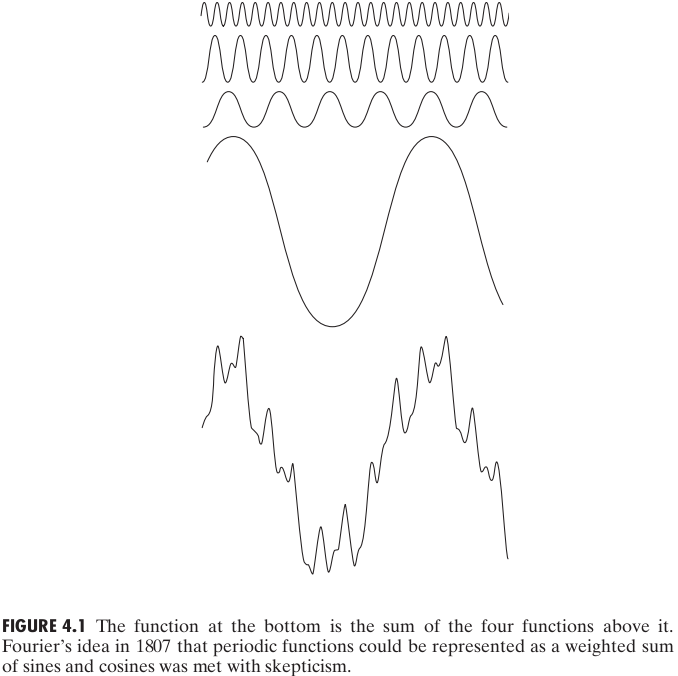
\includegraphics[width=.6\textwidth]{fig-4-1}
\end{figure}
\end{frame}

%----------------------------------------------------------------------------------------

\subsection{Fourier Series}

%----------------------------------------------------------------------------------------

\begin{frame}
\frametitle{Fourier Series}
A function $f(t)$ periodic with period $T$, can be expressed as the sum of sines and cosines multiplied
by appropriate coefficients.
\begin{equation}
\boxed{
f(t) =
\sum_{n=-\infty}^{\infty}
c_{n}
e^{j\dfrac{2\pi n}{T}t}
}
\end{equation}
where the coefficients are given by
\begin{equation}
\boxed{
c_{n} = \dfrac{1}{T}
\int_{-T/2}^{T/2}
f(t)
e^{-j\dfrac{2\pi n}{T}t}
dt
}
,
\end{equation}
for $n=0,\pm 1, \pm 2, \ldots$
\end{frame}

%----------------------------------------------------------------------------------------

\begin{frame}
Using the Euler formula:
\begin{equation}
e^{j\theta} = \cos\theta + j\sin\theta
\end{equation}
The representation of $f(t)$ in Fourier series can be expanded as:
\begin{equation}
f(t) =
\sum_{n=-\infty}^{\infty}
c_{n}
\left [
\cos \left ( \dfrac{2\pi n}{T}t \right ) +
j\sin \left ( \dfrac{2\pi n}{T}t \right )
\right ]
\end{equation}
\end{frame}

%----------------------------------------------------------------------------------------

\begin{frame}
Example 1:
\begin{columns}
\begin{column}{.5\textwidth}
\begin{figure}
\centering
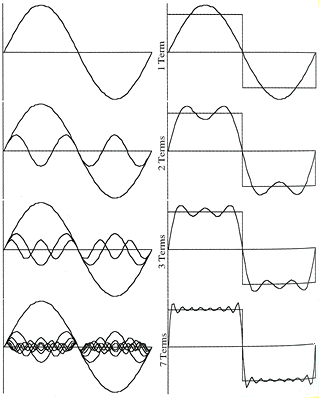
\includegraphics[width=\textwidth]{fourier_series}
\end{figure}
\end{column}
\begin{column}{.5\textwidth}
\[
f_{1}(x) = \sin(2\pi ft).
\]
\[
f_{2}(x) = \sin(2\pi ft) + (1/3)\sin(6\pi ft).
\]
\[
\begin{split}
f_{3}(x) = & \sin(2\pi ft) + \\
&(1/3)\sin(6\pi ft) + \\
& (1/5)\sin(10\pi ft).
\end{split}
\]
\[
\begin{split}
f_{4}(x) = & \sin(2\pi ft) + (1/3)\sin(6\pi ft) + \\
& (1/5)\sin(10\pi ft) + \\
&(1/7)\sin(14\pi ft) + \\
& (1/9)\sin(18\pi ft) + \\
&(1/11)\sin(22\pi ft) + \\
& (1/13)\sin(26\pi ft).
\end{split}
\]
\end{column}
\end{columns}
\end{frame}

%----------------------------------------------------------------------------------------

\begin{frame}
Example 2:
\begin{figure}
\centering
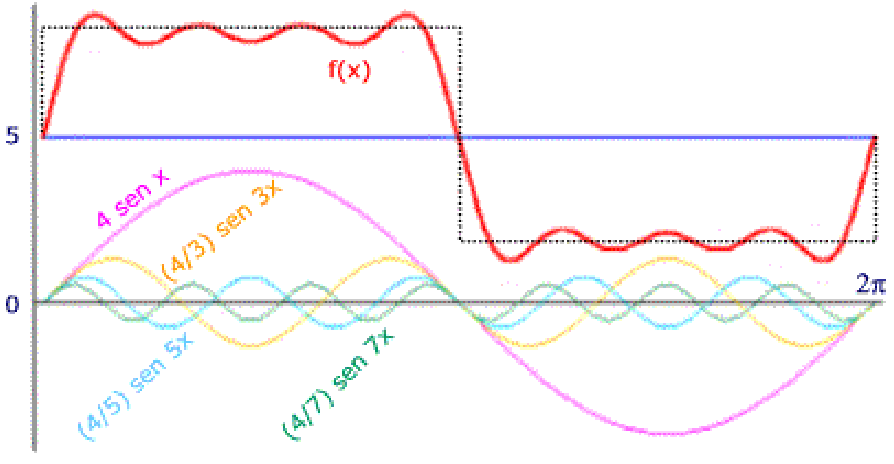
\includegraphics[width=\textwidth]{square-wave}
\end{figure}
\end{frame}

%----------------------------------------------------------------------------------------

\begin{frame}
Note:
\begin{itemize}
\item First component $c_{0} = 5$ is the signal's \textit{dc}\footnote{\textit{Direct current}} component.
\item Second component $4\sin x$ is the \textit{fundamental frequency}, since it has the same frequency as the signal.
\item Next components ($\sin 3x,\ \sin 5x, \ldots$) are the signal's \textit{harmonics}.
\item Every periodic signal is formed by
\begin{itemize}
\item A \textit{dc} component.
\item A harmonic signal.
\item Harmonic components.
\end{itemize}
\end{itemize}
\end{frame}

%----------------------------------------------------------------------------------------

\begin{frame}
\begin{itemize}
\item Coefficients $c_{n}$ are the amplitudes of the harmonics.
\item Frequency spectrum containing the first 25 harmonics:
\end{itemize}
\begin{figure}
\centering
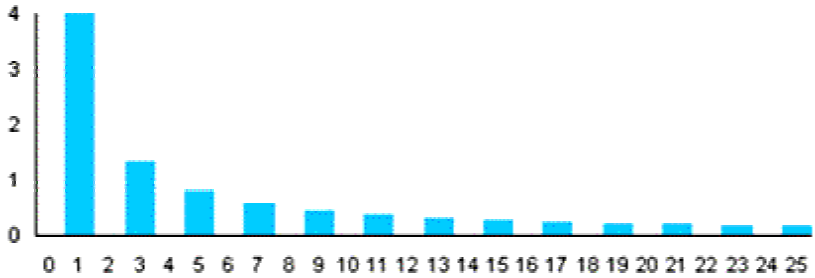
\includegraphics[width=\textwidth]{square-wave-2}
\end{figure}
\end{frame}

%----------------------------------------------------------------------------------------

\subsection{Impulses}

%----------------------------------------------------------------------------------------

\begin{frame}
\frametitle{Impulses}
A unit impulse of a continuous variable located at $t=0$ denoted is \textit{defined} as
\begin{equation}
\delta(t) = \left \{
\begin{array}{ll}
\infty, & \text{if } t=0\\
0		& \text{if } t\neq 0
\end{array}
\right .
\end{equation}
and satisfies
\begin{equation}
\int_{-\infty}^{\infty} \delta(t) dt = 1.
\end{equation}
\end{frame}

%----------------------------------------------------------------------------------------

\begin{frame}
An impulse can be viewed as a spike occurring at $t=0$ of:

\begin{columns}
\begin{column}{.3\textwidth}
\begin{itemize}
\item Infinite amplitude.
\item Zero duration.
\item Unit area.
\end{itemize}
\end{column}
\begin{column}{.7\textwidth}
\begin{figure}
\centering
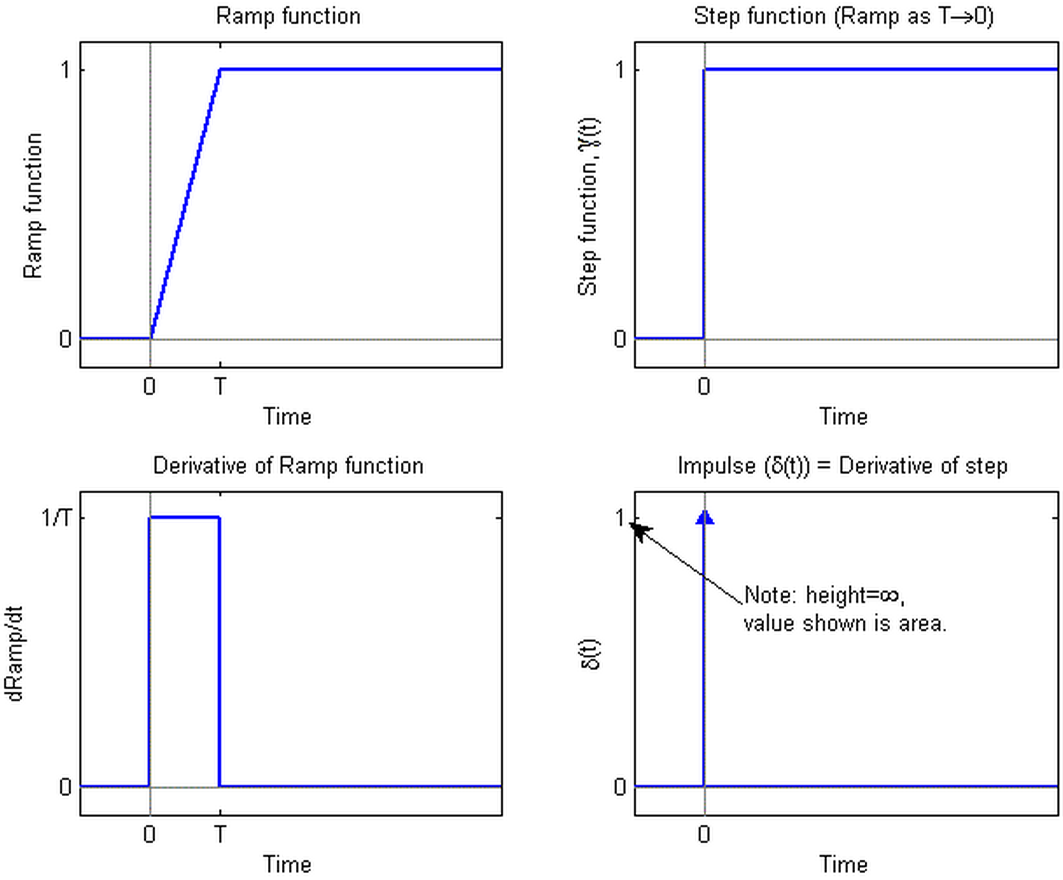
\includegraphics[width=\textwidth]{impulse}
\end{figure}
\end{column}
\end{columns}
\end{frame}

%----------------------------------------------------------------------------------------

\begin{frame}
Sifting property:
\begin{equation}
\int_{-\infty}^{\infty} f(t)\delta(t) dt = f(0)
\end{equation}
Sifting simply yields the value of the function (t) at the location of the impulse.\\
More generally:
\begin{equation}
\boxed{\int_{-\infty}^{\infty} f(t) \delta(t-t_{0}) dt = f(t_{0})}.
\end{equation}
\end{frame}

%----------------------------------------------------------------------------------------

\begin{frame}
The unit discrete impulse $\delta(x)$:
\begin{equation}
\delta(x) = \left \{
\begin{array}{ll}
1 & x=0\\
0 & x\neq 0
\end{array}
\right .
\end{equation}
Also:
\begin{equation}
\sum_{x=-\infty}^{\infty} \delta(x) = 1.
\end{equation}
And the sifting property:
\begin{equation}
\sum_{x=-\infty}^{\infty}f(x) \delta(x-x_{0}) = f(x_{0}).
\end{equation}
\end{frame}

%----------------------------------------------------------------------------------------

\begin{frame}
The \textit{impulse train} is defined as the sum of infinitely many periodic impulses $\Delta T$ apart:
\begin{equation}
s_{\Delta T}(t) = \sum_{n=-\infty}^{\infty}\delta(t-n\Delta T).
\end{equation}
\begin{figure}
\centering
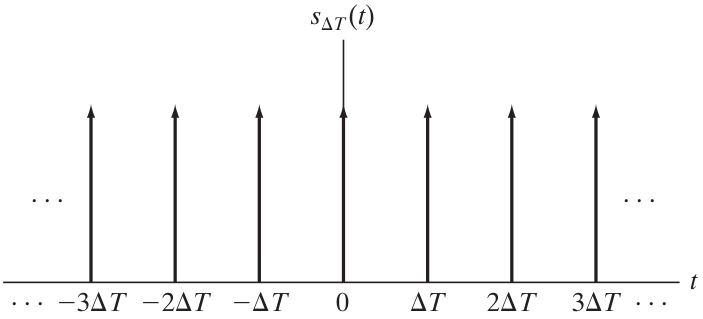
\includegraphics[width=.6\textwidth]{fig-4-3}
\end{figure}
The impulse train is important to understand the \textit{sampling} process and its properties.
\end{frame}

%----------------------------------------------------------------------------------------

\subsection{Fourier Transform}

%----------------------------------------------------------------------------------------

\begin{frame}
\frametitle{Fourier Transform}
The Fourier transform of a continuous function $f(t)$ of a continuous variable $t$, is defined by the equation
\begin{equation}
\boxed{
\mathcal{F}\left \{ f(t) \right \} = F(\mu) = \int_{-\infty}^{\infty} f(t) e^{-j2\pi \mu t} dt
},
\end{equation}
Conversely, given $F(\mu)$;
\begin{equation}
\boxed{
f(t) = \mathcal{F}^{-1}\{F(\mu)\} = \int_{-\infty}^{\infty} F(\mu) e^{j2\pi \mu t} d\mu
}.
\end{equation}
These two equations comprise the \textit{Fourier transform pair}.
\end{frame}

%----------------------------------------------------------------------------------------

\begin{frame}
Using Euler's formula:
\begin{equation}
\begin{split}
F(\mu) = & \int_{-\infty}^{\infty} f(t) e^{-j2\pi \mu t} dt \\
&= \int_{-\infty}^{\infty} f(t) [ \cos(2\pi \mu t) + j\sin(2\pi \mu t) ]
\end{split}
\end{equation}
\begin{itemize}
\item The Fourier transform is an expansion of $f(t)$ multiplied by sinusoidal terms whose frequencies are determined by the values of $\mu$.
\item After integration, only the frequency remains, so the domain of the Fourier transform is called the \textit{frequency} domain (cycles per second).
\end{itemize}
\end{frame}

%----------------------------------------------------------------------------------------

\begin{frame}
The Fourier transform of a real function is, in general, complex:
\begin{itemize}
\item Fourier spectrum:
\begin{equation}
|F(\mu)| = \left [R^{2}(\mu) + I^{2}(\mu) \right ]^{1/2}.
\end{equation}
\item Phase:
\begin{equation}
\phi(\mu) = \tan^{-1}\left [ \dfrac{I(\mu)}{R(\mu)} \right ].
\end{equation}
\item Power spectrum:
\begin{equation}
P(\mu) = |F(\mu)|^{2} = R^{2}(\mu) + I^{2}(\mu).
\end{equation}
\end{itemize}
\end{frame}

%----------------------------------------------------------------------------------------
%
%\begin{frame}
%The Fourier transform of a real function is, in general, complex:
%\[
%F(\mu) = R(\mu) + jI(\mu)
%\]
%\[
%F(\mu) = \left | F(\mu) \right | e^{j\phi(\mu)}
%\]
%\[
%|F(\mu)| = \left [R^{2}(\mu) + I^{2}(\mu) \right ]^{1/2} 
%\]
%\[
%\phi(\mu) = \tan^{-1}\left [ \dfrac{I(\mu)}{R(\mu)} \right ]
%\]
%\end{frame}

%----------------------------------------------------------------------------------------

\begin{frame}
\frametitle{Example 1: The Fourier transform of a simple function}
\begin{equation*}
f(t) =
\left \{
\begin{array}{ll}
A, & |t| < W/2 \\
0, & \text{otherwise}
\end{array}
\right .
\end{equation*}
\end{frame}

%----------------------------------------------------------------------------------------

\begin{frame}
\frametitle{Example 1: The Fourier transform of a simple function}
\begin{columns}
\begin{column}{.5\textwidth}
\begin{figure}
\centering
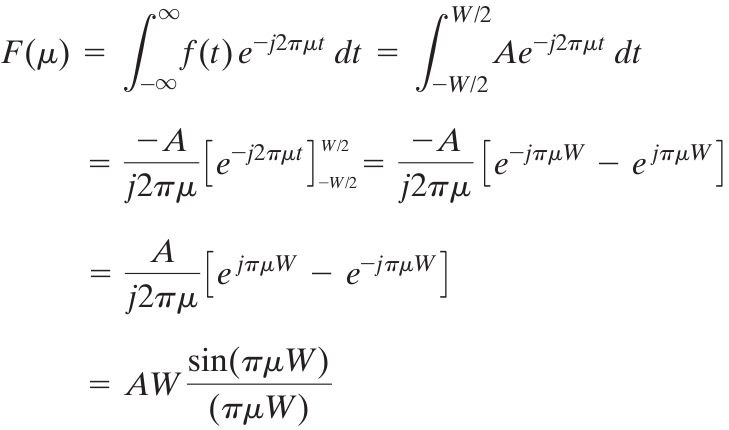
\includegraphics[width=\textwidth]{ex-4-1}
\end{figure}
\end{column}
\begin{column}{.5\textwidth}
The magnitude of the transform is commonly used:
\begin{equation}
|F(\mu)| = AT\left | \dfrac{\sin(\pi \mu W)}{\pi\mu W} \right |
\end{equation}
\end{column}
\end{columns}
\begin{figure}
\centering
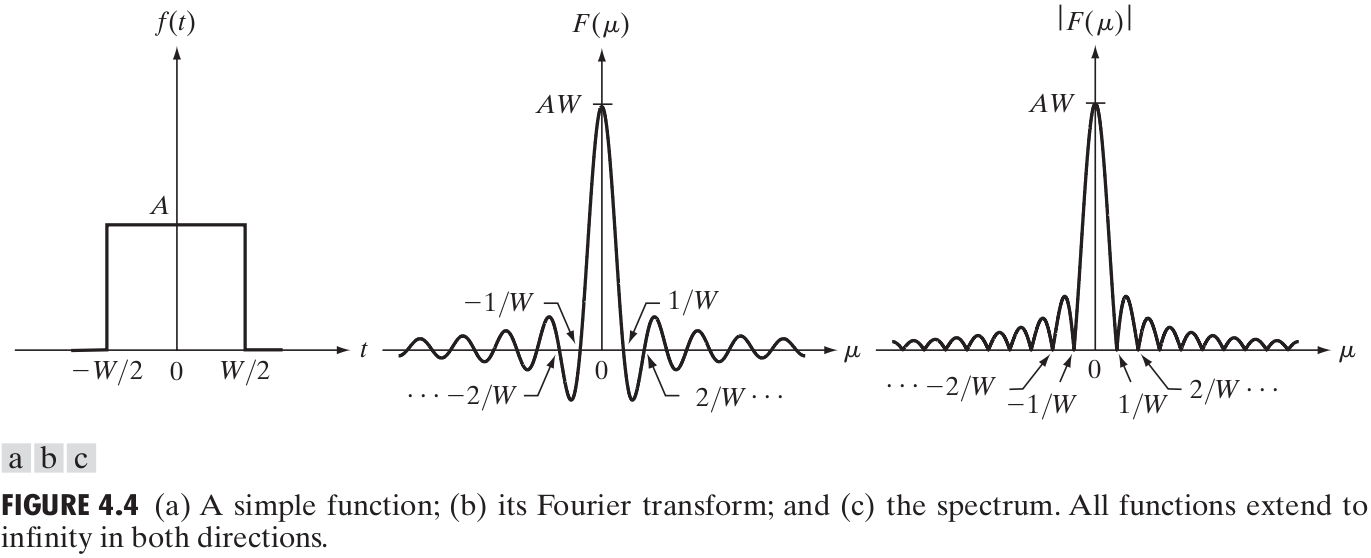
\includegraphics[width=.7\textwidth]{fig-4-4}
\end{figure}
\end{frame}

%----------------------------------------------------------------------------------------

\begin{frame}
\frametitle{Example 1: The Fourier transform of a simple function}
\begin{itemize}
\item The zeros in $|F(\mu)|$ are inversely proportional to the width $W$.
\end{itemize}
\begin{figure}
\centering
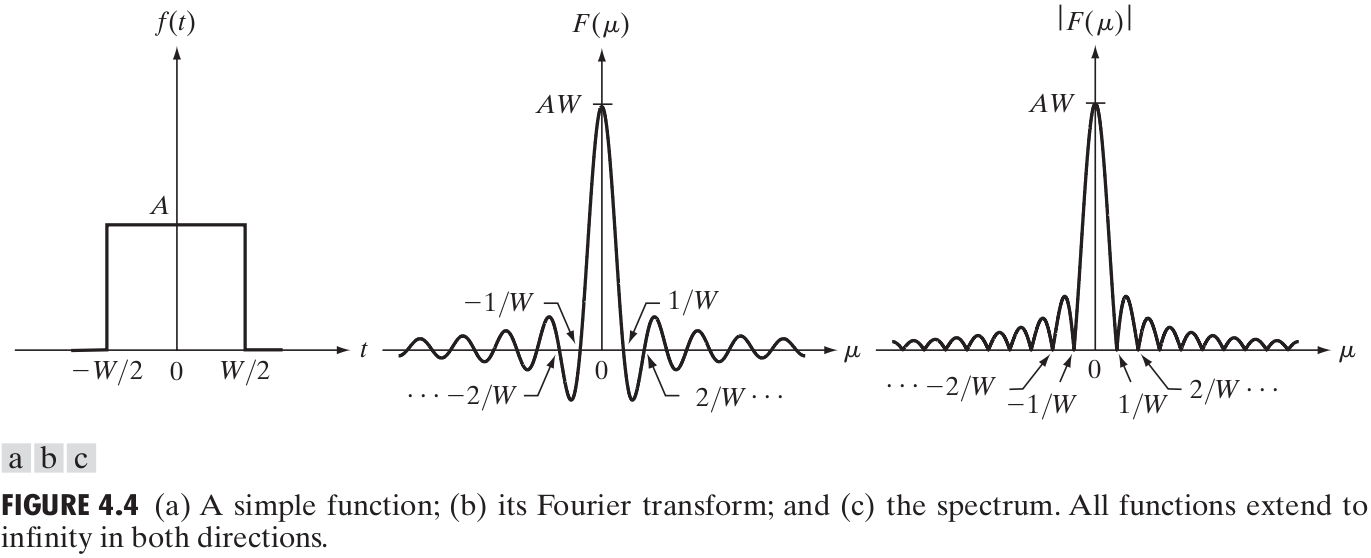
\includegraphics[width=.8\textwidth]{fig-4-4}
\end{figure}
\end{frame}

%----------------------------------------------------------------------------------------

\begin{frame}
\frametitle{Example 2: The Fourier transform of the impulse}
\begin{equation*}
\delta(t) = \left \{
\begin{array}{ll}
\infty, & \text{if } t=0\\
0		& \text{if } t\neq 0
\end{array}
\right .
\end{equation*}
\end{frame}

%----------------------------------------------------------------------------------------

\begin{frame}
\frametitle{Example 2: The Fourier transform of the impulse}
\begin{figure}
\centering
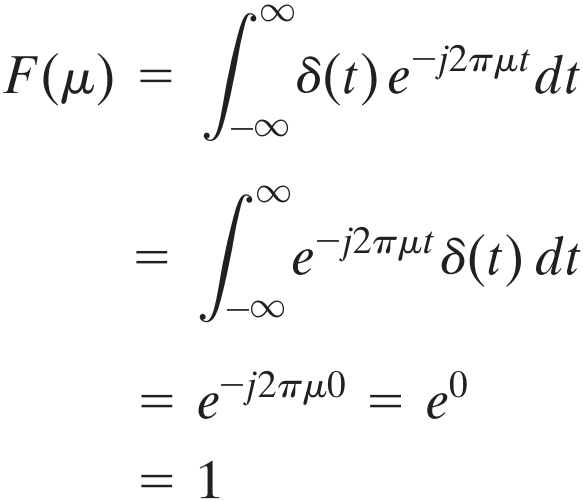
\includegraphics[width=.3\textwidth]{ex-4-2}
\end{figure}
\begin{block}{}
The Fourier transform of an impulse located at the origin of the spatial domain is a constant in the frequency domain.
\end{block}
\end{frame}

%----------------------------------------------------------------------------------------

\begin{frame}
\frametitle{Example 3: The Fourier transform of a shifted impulse}
\begin{figure}
\centering
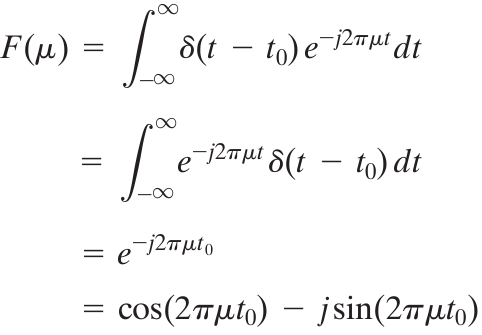
\includegraphics[width=.4\textwidth]{ex-4-2_2}
\end{figure}
\begin{block}{}
The last two lines are equivalent representations of a unit circle centered on the origin of the complex plane.
\end{block}
\end{frame}

%----------------------------------------------------------------------------------------

\begin{frame}
\frametitle{Example 4: The Fourier transform of the impulse train}
\begin{block}{Step 1}
Use Fourier series to represent the impulse train
\end{block}
\[
s_{\Delta T}(t) =
\sum_{n=-\infty}^{\infty}
c_{n}
e^{j2\pi(n/\Delta T)t}
\]

\[
c_{n} = \dfrac{1}{\Delta T}
\int_{-\Delta T/2}^{\Delta T/2}
s_{\Delta T}(t)
e^{-j2\pi(n/\Delta T)t}
dt = \dfrac{1}{\Delta T}
\]
i. e.,
\[
\boxed{
s_{\Delta T}(t) = \dfrac{1}{\Delta T}
\sum_{n=-\infty}^{\infty}
e^{j2\pi(n/\Delta T)t}
}
\]
\end{frame}

%----------------------------------------------------------------------------------------

\begin{frame}
\begin{block}{Step 2}
Consider the Fourier transform of the shifted impulse
\end{block}
\begin{equation}
\delta(t-t_{0}) \leftrightharpoons e^{-j2\pi \mu t_{0}}
\end{equation}
\end{frame}

%----------------------------------------------------------------------------------------

\begin{frame}
\begin{block}{Step 3}
Use symmetry to find the Fourier transform of the complex exponential, based on the Fourier transform of the impulse
\end{block}
\begin{block}{Symmetry property}
If $f(t)\leftrightharpoons F(\mu)$, then $F(t) \leftrightharpoons f(-t)$
\end{block}
I. e., if $\delta(t-t_{0}) \leftrightharpoons e^{-j2\pi \mu t_{0}}$, we have
\[
e^{-j2\pi t_{0} t} \leftrightharpoons \delta(-\mu-t_{0})
\]
make $-t_{0} = a$
\[
\boxed{
e^{j2\pi at} \leftrightharpoons \delta(-\mu+a) = \delta(\mu-a)
}
\]
\end{frame}

%----------------------------------------------------------------------------------------

\begin{frame}
\begin{block}{Step 4}
From the Fourier series representation of the impulse train, use the results of steps 2 and 3 to obtain the Fourier transform of the impulse train
\end{block}
\begin{equation}
\begin{split}
s_{\Delta T}(t) = & \dfrac{1}{\Delta T}
\sum_{n=-\infty}^{\infty}
e^{j2\pi(n/\Delta T)t} \\
& \leftrightharpoons \dfrac{1}{\Delta T} \sum_{n=-\infty}^{\infty} \delta(\mu - n/\Delta T).
\end{split}
\end{equation}
\begin{block}{The Fourier transform $\ldots$}
$\ldots$ of an impulse train with period $\Delta T$ is also an impulse train, whose period is $1/\Delta T$.
\end{block}
\end{frame}

%----------------------------------------------------------------------------------------

\subsection{Convolution}

%----------------------------------------------------------------------------------------

\begin{frame}
\frametitle{Convolution}
\begin{itemize}
\item The convolution of two functions involves flipping (rotating by $180^{\circ}$) one function about its origin and sliding it past the other.
\item In the convolution of two continuous functions $f(t)$ and $h(t)$, the sum of products reduces to the integral:
\begin{equation}
f(t) \star h(t) = \int_{-\infty}^{\infty} f(\tau)h(t-\tau) d\tau.
\end{equation}
where:
\begin{itemize}
\item $t$ is the \textit{displacement}.
\item $\tau$ is a dummy variable.
\item The minus sign does the rotation.
\end{itemize}
\end{itemize}
\end{frame}

%----------------------------------------------------------------------------------------

\begin{frame}
Given the following property:
\begin{block}{Displacement property of the Fourier transform}
If $h(t) \leftrightharpoons H(\mu)$, then
\begin{equation}
h(t-\tau) = e^{-j2\pi \mu\tau} H(\mu).
\end{equation}
\end{block}
Let's compute the Fourier transform of the convolution integral:
\end{frame}

%----------------------------------------------------------------------------------------

\begin{frame}
The Fourier transform of the convolution integral is given by
\begin{equation}
\begin{split}
\mathcal{F} \left \{ f(t) \star h(t) \right \} = & \mathcal{F} \left \{ \int_{-\infty}^{\infty} f(t) h(t-\tau) d\tau \right \} \\
= & \int_{-\infty}^{\infty} \left [ \int_{-\infty}^{\infty} f(\tau) h(t-\tau) d\tau \right ] e^{-j2\pi \mu t} dt \\
= & \int_{-\infty}^{\infty} f(\tau) \left [ \int_{-\infty}^{\infty} h(t-\tau) e^{-2j\pi \mu t} dt \right ] d\tau \\
= & \int_{-\infty}^{\infty} f(\tau) \left [ e^{-j2\pi \mu\tau} H(\mu) \right ] d\tau\\
= & H(\mu) \int_{-\infty}^{\infty} f(\tau) e^{-j2\pi \mu\tau} d\tau \\
= & H(\mu)F(\mu)
\end{split}
\end{equation}
\end{frame}

%----------------------------------------------------------------------------------------

\begin{frame}
\begin{block}{The convolution theorem}
\begin{itemize}
\item The Fourier transform of the convolution of two functions in the spatial domain is equal to the product in the frequency domain of the Fourier transforms of the two functions.
\begin{equation}
\boxed{
f(t) \star h(t) \leftrightharpoons F(\mu) H(\mu)
}
\end{equation}
\item Equivalently; the convolution in the frequency domain is analogous to multiplication in the spatial domain:
\begin{equation}
\boxed{
f(t)h(t) \leftrightharpoons F(\mu) \star H(\mu)
}
\end{equation}
\end{itemize}
\end{block}
\end{frame}

%----------------------------------------------------------------------------------------

\section{Sampling}

%----------------------------------------------------------------------------------------

\begin{frame}
Sampling:
\begin{figure}
\centering
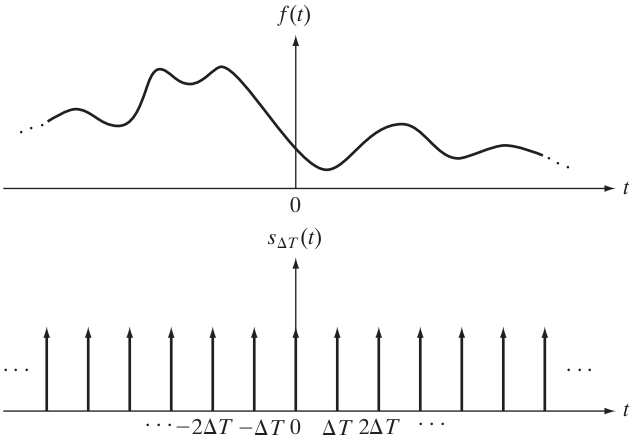
\includegraphics[width=.4\textwidth]{fig-4-5-a-b}
\end{figure}
\begin{figure}
\centering
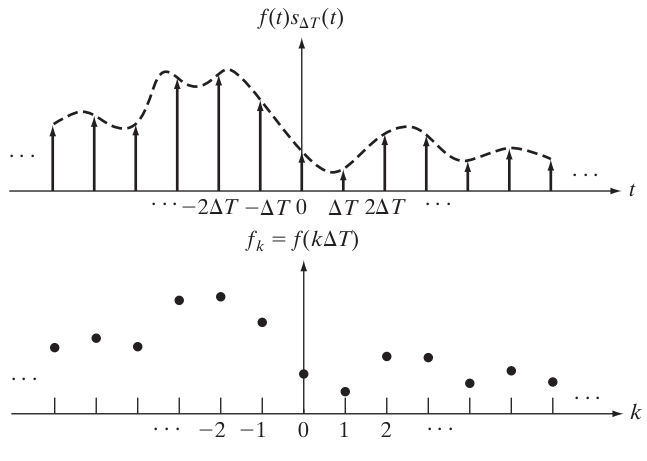
\includegraphics[width=.4\textwidth]{fig-4-5-c-d}
\end{figure}
\end{frame}

%----------------------------------------------------------------------------------------

\begin{frame}
The sampled function $\tilde{f}(t)$ is modeled by the product of the function $f(t)$ with the impulse train:
\begin{equation}
\tilde{f}(t) = f(t)\cdot s_{\Delta T} (t) =  \sum_{n=-\infty}^{\infty} f(t) \delta(t - n\Delta T)
\end{equation}
Each component of this summation is an impulse weighted by the value of $f(t)$ at the location of the impulse:
\begin{equation}
\begin{split}
f_{k} = & \int_{-\infty}^{\infty} f(t) \delta(t-k\Delta T) dt \\
= & f(k\Delta T).
\end{split}
\end{equation}
\end{frame}

%----------------------------------------------------------------------------------------

\subsection{The Fourier transform of sampled functions}

%----------------------------------------------------------------------------------------

\begin{frame}
Since the Fourier transform of the product of two functions
in the spatial domain is the convolution of the transforms of the two functions in the frequency domain, we have:
\begin{equation}
f(t) s_{\Delta T}(t) \leftrightharpoons F(\mu) \star S(\mu)
\end{equation}
And since $s_{\Delta T}(t) \leftrightharpoons \dfrac{1}{\Delta T} \sum_{n=-\infty}^{\infty} \delta(\mu - n/\Delta T)$
we have that
\end{frame}

%----------------------------------------------------------------------------------------

\begin{frame}
\begin{figure}
\centering
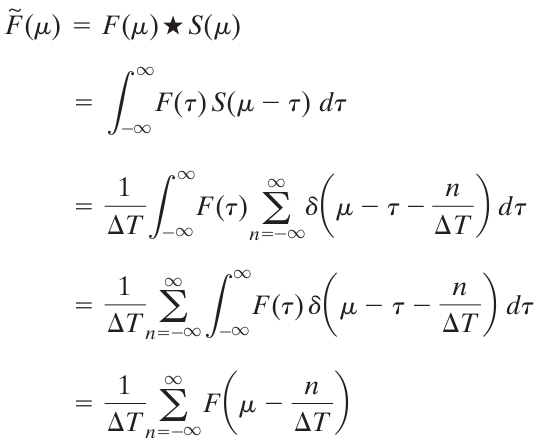
\includegraphics[width=.6\textwidth]{eq-4-3-5}
\end{figure}
I. e., the Fourier transform of the sampled function is an infinite, periodic sequence of copies of the transform of the original, continuous function.
\end{frame}

%----------------------------------------------------------------------------------------

\begin{frame}
\begin{figure}
\centering
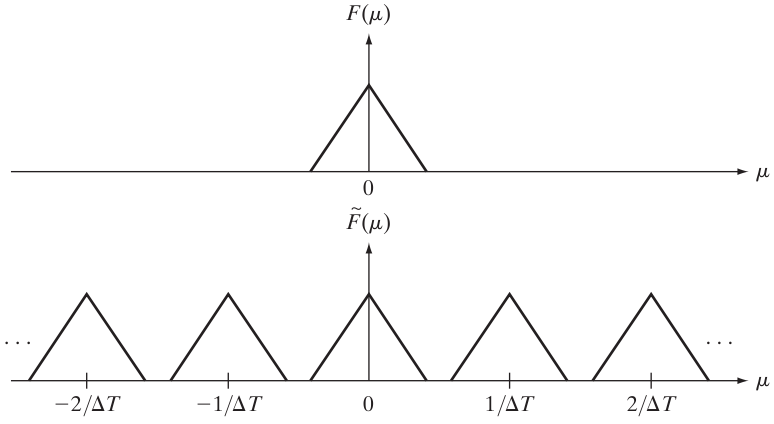
\includegraphics[width=.6\textwidth]{fig-4-6-a-b}
\end{figure}
\begin{figure}
\centering
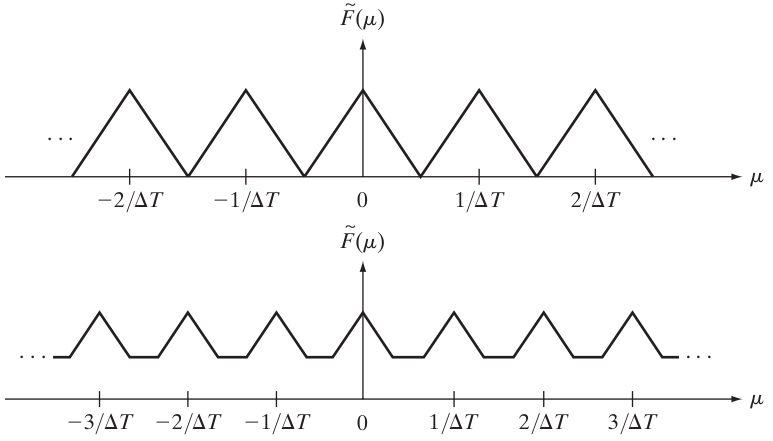
\includegraphics[width=.6\textwidth]{fig-4-6-c-d}
\end{figure}
\end{frame}

%----------------------------------------------------------------------------------------

\subsection{The sampling theorem}

%----------------------------------------------------------------------------------------

\begin{frame}
\begin{columns}
\begin{column}{.5\textwidth}
\begin{itemize}
\item A function $f(t)$ is band limited if $F(\mu) =0$ outside an interval $[-\mu_{min}, \mu_{max}]$.
\item If one period of the Fourier transform of the sampled function $\tilde{F}(\mu)$ can be isolated, we can recover $f(t)$ computing its inverse Fourier transform!
\end{itemize}
\end{column}
\begin{column}{.5\textwidth}
\begin{figure}
\centering
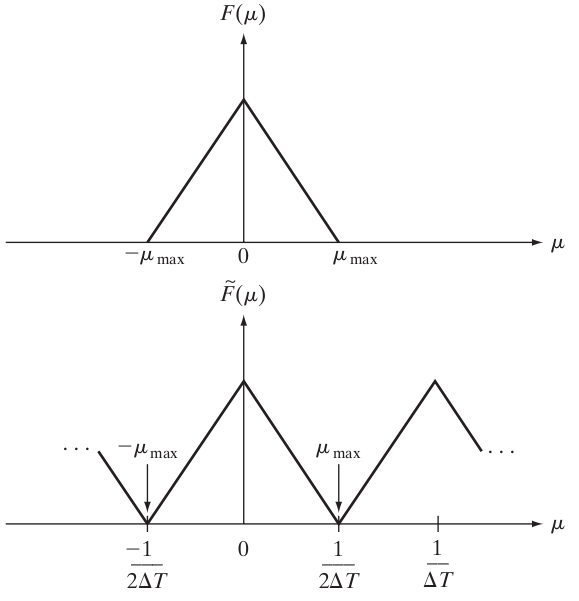
\includegraphics[width=\textwidth]{fig-4-7}
\end{figure}
\end{column}
\end{columns}
\end{frame}

%----------------------------------------------------------------------------------------

\begin{frame}
\begin{columns}
\begin{column}{.5\textwidth}
\begin{itemize}
\item Sufficient separation is guaranteed if
\begin{equation}
\dfrac{1}{2\Delta T} \geq \mu_{max}.
\end{equation}
\end{itemize}
\begin{block}{\textit{Sampling theorem}}
The sampling frequency must be higher than twice the signal's highest frequency.
\end{block}
\end{column}
\begin{column}{.5\textwidth}
\begin{figure}
\centering
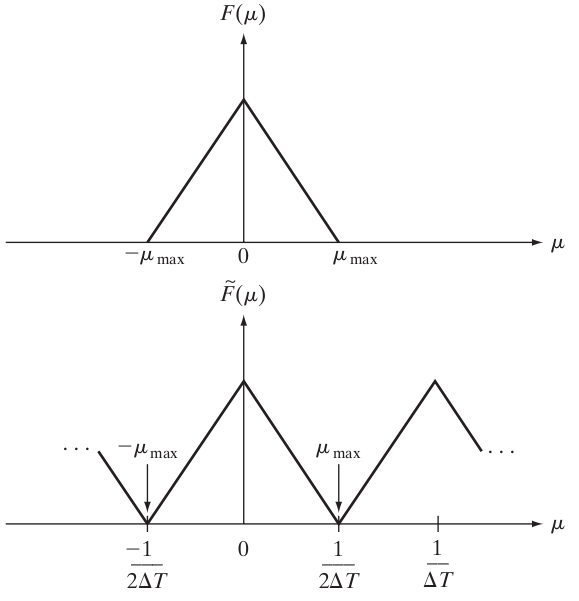
\includegraphics[width=\textwidth]{fig-4-7}
\end{figure}
\end{column}
\end{columns}
\end{frame}

%----------------------------------------------------------------------------------------

\begin{frame}
\begin{columns}
\begin{column}{.5\textwidth}
\begin{itemize}
\item Equivalently, sampling a signal with $1/\Delta T$ allow to ``capture'' a highest frequency equals $1/(2\Delta T)$.
\end{itemize}
\begin{block}{\textit{The Nyquist rate}}
The Nyquist rate equals exactly twice the signal's highest frequency.
\end{block}
\end{column}
\begin{column}{.5\textwidth}
\begin{figure}
\centering
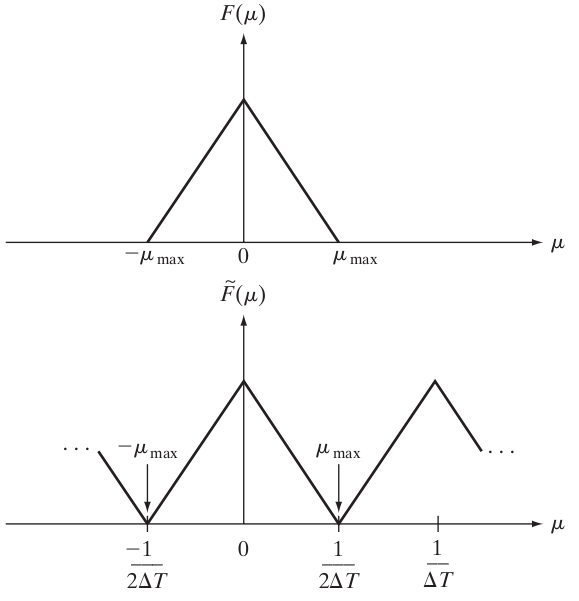
\includegraphics[width=\textwidth]{fig-4-7}
\end{figure}
\end{column}
\end{columns}
\end{frame}

%----------------------------------------------------------------------------------------

\begin{frame}
\begin{columns}
\begin{column}{.6\textwidth}
\begin{figure}
\centering
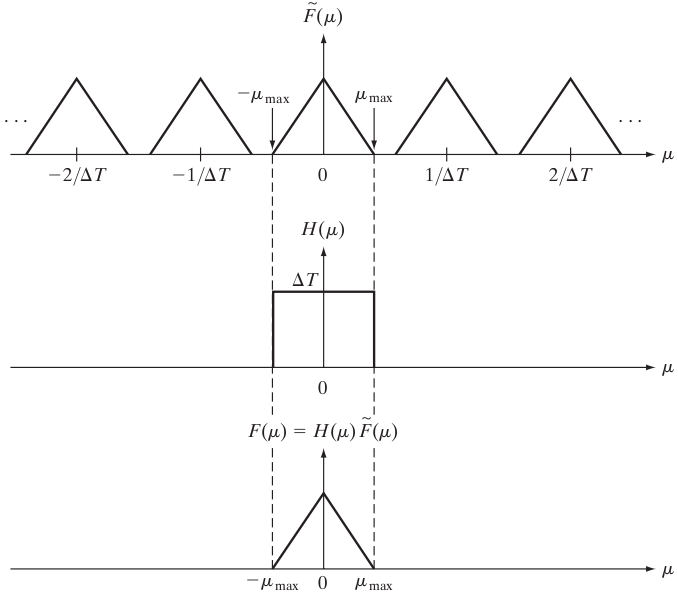
\includegraphics[width=\textwidth]{fig-4-8}
\end{figure}
\end{column}
\begin{column}{.4\textwidth}
\begin{enumerate}
\item Sample $f(t)$ to obtain $\tilde{F}(\mu)$.
\item Filter $\tilde{F}(\mu)$ to obtain
\begin{equation}
F(\mu) = H(\mu)F(\mu)\notag
\end{equation}
\item Recover $f(t)$ using
\begin{equation}
f(t) = \mathcal{F}^{-1}\{F(\mu)\}\notag
\end{equation}
\end{enumerate}
\end{column}
\end{columns}
\end{frame}

%----------------------------------------------------------------------------------------

\subsection{Aliasing}

%----------------------------------------------------------------------------------------

\begin{frame}
\frametitle{Aliasing}
\begin{columns}
\begin{column}{.3\textwidth}
Happens when a band-limited function is sampled at a rate smaller than twice its highest frequency.
\end{column}
\begin{column}{.7\textwidth}
\begin{figure}
\centering
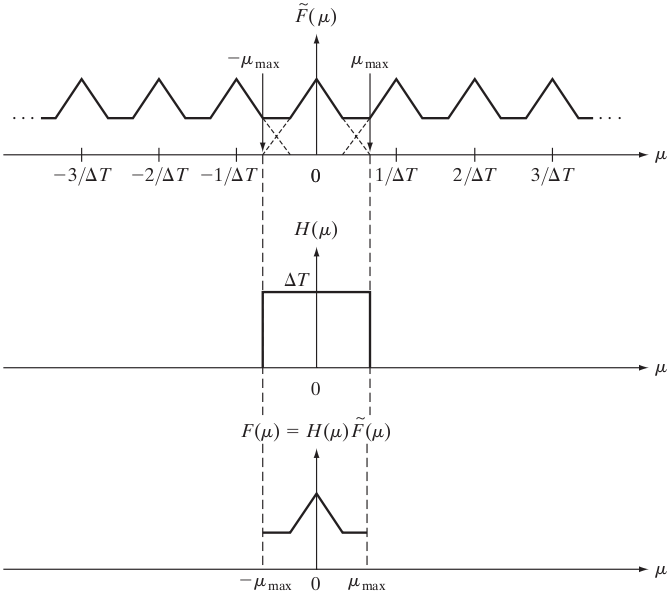
\includegraphics[width=.9\textwidth]{fig-4-9}
\end{figure}
\end{column}
\end{columns}
\end{frame}

%----------------------------------------------------------------------------------------

\begin{frame}
\begin{block}{Aliasing}
Aliasing is a process in which
high frequency components of a continuous function ``masquerade'' as lower frequencies in the sampled function.
\end{block}
\end{frame}

%----------------------------------------------------------------------------------------

\begin{frame}
Aliasing:
\begin{itemize}
\item \textbf{Is always present} because, in practice, the function must have limited duration.
\end{itemize}
Limiting duration implies:
\begin{itemize}
\item multiplying $f(t)$ by
\[
h(t) = \left \{
\begin{array}{ll}
1, & 0\leq t \leq T \\
0, & \text{otherwise}
\end{array}
\right .
\]
which implies;
\item making the convolution $F(\mu)\star H(\mu)$, where $H(\mu)$ is the infinite sinc function.
\end{itemize}
\end{frame}

%----------------------------------------------------------------------------------------

\begin{frame}
\begin{itemize}
\item Having to limit the duration of a function prevents its perfect recover using sampling.
\item Aliasing is inevitable!
\end{itemize}
\begin{block}{\textit{Anti-aliasing}}
Aliasing can be \textit{reduced} by \textit{smoothing} the input function to attenuate its higher frequencies \textbf{prior} to sampling.
\end{block}
\end{frame}

%----------------------------------------------------------------------------------------

\begin{frame}
\frametitle{Example}
\begin{itemize}
\item Infinite band-limited $f(t)=\sin(\pi t)$.
\item $\mu_{max} = 0.5$~Hz, i. e., $\Delta T < 1s$ is required.
\item What happens if $\Delta T = 1s$?
\item With $\Delta T \gtrsim 2$ The frequency of the dots is approximately one tenth of $f(t)$.
\end{itemize}
\begin{figure}
\centering
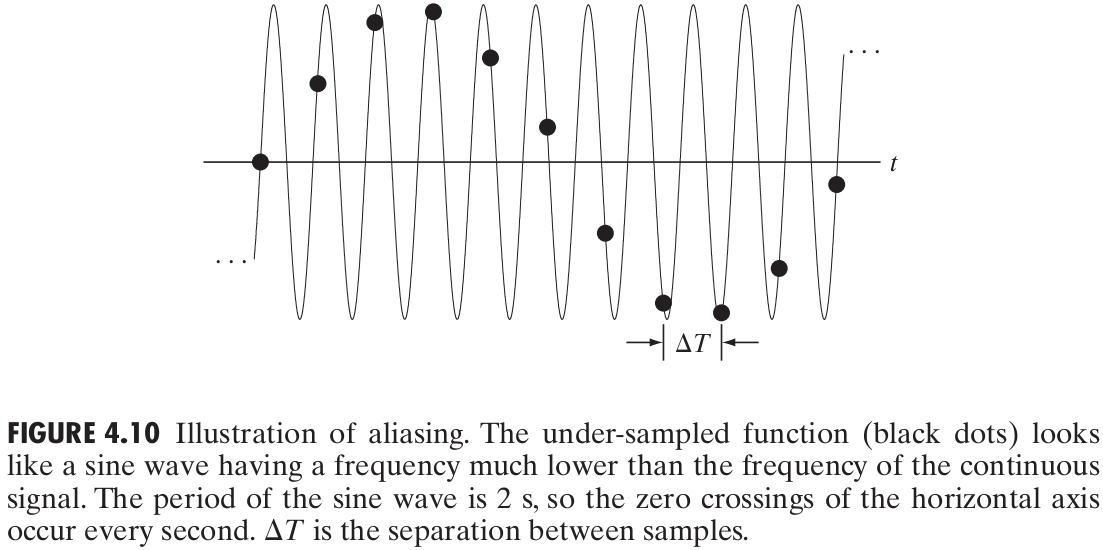
\includegraphics[width=.6\textwidth]{fig-4-10}
\end{figure}
\end{frame}

%----------------------------------------------------------------------------------------

\subsection{Recovery from sample data}

%----------------------------------------------------------------------------------------

\begin{frame}
\frametitle{Sampling representation in the spatial domain}
\begin{equation}
f (t) \leftrightharpoons F(\mu) = \tilde{F}(\mu) H(\mu) = h(t) \star \tilde{F}(\mu)
\end{equation}
Remembering that
\[
\tilde{f}(t) = f(t)\cdot s_{\Delta T} (t) =  \sum_{n=-\infty}^{\infty} f(t) \delta(t - n\Delta T)
\]
and
\[
f(t) \star h(t) = \int_{-\infty}^{\infty} f(\tau)h(t-\tau) d\tau
\]
we have
\begin{equation}
\boxed{
f(t) = \sum_{n=-\infty}^{\infty} f(n\Delta T) \text{sinc}\left [ \dfrac{t - n\Delta T}{n\Delta T} \right ]
}
\end{equation}
\end{frame}

%----------------------------------------------------------------------------------------

\begin{frame}
Sampling in the spatial domain:
\begin{columns}
\begin{column}{.5\textwidth}
\begin{equation}
f(t) = \sum_{n=-\infty}^{\infty} f(n\Delta T) \text{sinc}\left [ \dfrac{t - n\Delta T}{n\Delta T} \right ] \notag
\end{equation}
\end{column}
\begin{column}{.5\textwidth}
\begin{figure}
\centering
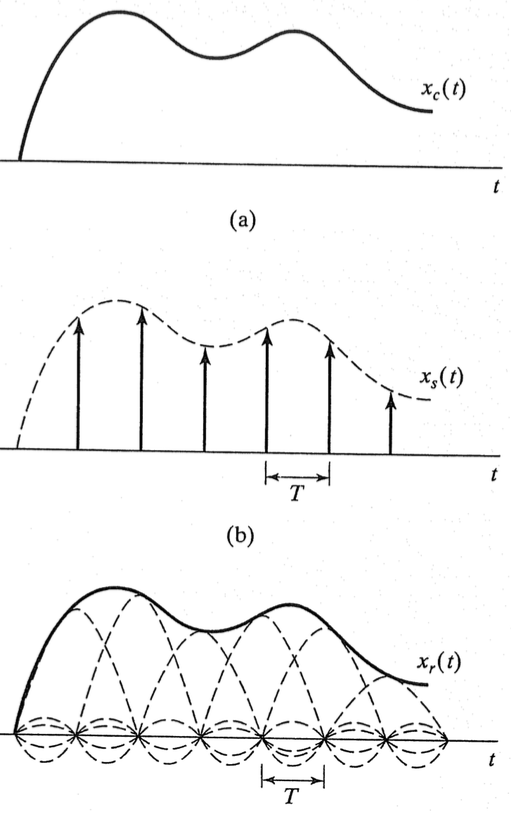
\includegraphics[width=.8\textwidth]{amostragem-sinc}
\end{figure}
\end{column}
\end{columns}
\end{frame}

\begin{frame}
\begin{itemize}
\item The perfectly reconstructed function is an infinite sum of sinc functions weighted by the sample values, and has the important property that the reconstructed function is identically equal to the sample values at multiple integer increments of $\Delta T$.
\item Previous equation requires an infinite number of terms for the interpolations between samples. In practice, this implies that we have to look for approximations that are finite interpolations between samples.
\end{itemize}
\end{frame}

%----------------------------------------------------------------------------------------

\section{The 1-D Discrete Fourier Transform (DFT)}

%----------------------------------------------------------------------------------------

\begin{frame}
\frametitle{Discrete Fourier Transform (DFT) of one variable}
We've seen that:
\begin{itemize}
\item The Fourier transform of a sampled, band-limited function $\tilde{f}(t)$ extending from $-\infty$ to $\infty$ is a;
\begin{itemize}
\item continuous;
\item periodic;
\end{itemize}
function $\tilde{F}(\mu)$ extending from $-\infty$ to $\infty$.
\item We know that
\[
\tilde{F}(\mu) = \sum_{n=-\infty}^{\infty} F\left ( \mu - \dfrac{n}{\Delta T} \right )
\]
but we want a way to compute $\tilde{F}(\mu)$ directly from $\tilde{f}(t)$.
\end{itemize}
\end{frame}

%----------------------------------------------------------------------------------------

\subsection{Obtaining the DFT from the continuous transform of a sampled function}

%----------------------------------------------------------------------------------------

\begin{frame}
Obtaining the DFT from the continuous Fourier transform of a sampled function.
\begin{equation}
\begin{split}
\tilde{F}(\mu) % = & \int_{-\infty}^{\infty} \tilde{f}(t) e^{-j2\pi \mu t}dt \\
= & \int_{-\infty}^{\infty} \left [ \sum_{n=-\infty}^{\infty} f(t)\delta(t-n\Delta T) \right ] e^{-j2\pi \mu t}dt \\
= & \sum_{n=-\infty}^{\infty} \int_{-\infty}^{\infty} f(t) \delta(t-n\Delta T) e^{-j2\pi \mu t}dt \\
= & \sum_{n=-\infty}^{\infty} f_{n} e^{-j2\pi \mu n\Delta T}
\end{split}
\end{equation}
where
\begin{equation}
f_{n} = \int_{-\infty}^{\infty} f(t) \delta(t - n\Delta T) dt.
\end{equation}
\end{frame}

%----------------------------------------------------------------------------------------

\begin{frame}
I. e.,
\begin{equation}
\boxed{
\tilde{F}(\mu) = \sum_{n=-\infty}^{\infty} f_{n} e^{-j2\pi \mu n\Delta T}
}
\end{equation}
Notice that, although $f_{n}$ is a discrete function, its Fourier transform $\tilde{F}(\mu)$ is:
\begin{itemize}
\item Continuous, and;
\item Infinitely periodic with period $1/\Delta T$.
\end{itemize}
Therefore, we need only one period of $\tilde{F}(\mu)$ to characterize it.
\end{frame}

%----------------------------------------------------------------------------------------

\begin{frame}
So:
\begin{itemize}
\item Obtain $M$ equally spaced samples of $\tilde{F}(\mu)$ over $\mu=0$ to $\mu=1/\Delta T$.
\item The samples occur at
\begin{equation}
\mu = \dfrac{m}{M\Delta T}, \qquad m = 0,1,2,\ldots, M-1.
\end{equation}
Resulting:
\end{itemize}
\begin{equation}
\boxed{
F_{m} = \sum_{n=0}^{M-1} f_{n} e^{-j2\pi mn/M}
},
\qquad m = 0,1,2,\ldots, M-1.
\end{equation}
\end{frame}

%----------------------------------------------------------------------------------------

\begin{frame}
This is the discrete Fourier transform pair:
\begin{equation}
\boxed{
F_{m} = \sum_{n=0}^{M-1} f_{n} e^{-j2\pi mn/M}
},
\qquad m = 0,1,2,\ldots, M-1.
\notag
\end{equation}
Conversely:
\begin{equation}
\boxed{
f_{n} = \dfrac{1}{M} \sum_{m=0}^{M-1} F_{m} e^{j2\pi nm/M}
},
\qquad n=0,1,\ldots,M-1.
\end{equation}
\end{frame}

%----------------------------------------------------------------------------------------

\begin{frame}
Notation change:
\begin{itemize}
\item So far, $t$ and $\mu$ were used to denote \textbf{continuous} spatial and frequency domains.
\item We'll use $(x,y)$ and $(u,v)$ to denote \textbf{discrete} spatial and frequency domains for two variables.
\item We'll also use $(t,z)$ and $(\mu, \nu)$ to denote \textbf{continuous} 2-D variables in the spatial and frequency domain, respectively.
\end{itemize}
\end{frame}

%----------------------------------------------------------------------------------------

\begin{frame}
The DFT pair becomes:
\begin{equation}
F(u) = \sum_{x=0}^{M-1} f(x) e ^{-j2\pi ux/M}\qquad u=0,1,\ldots,M-1.
\end{equation}
and
\begin{equation}
f(x) = \dfrac{1}{M} \sum_{u=0}^{M-1} F(u) e^{j2\pi ux/M}\qquad x=0,1,\ldots,M-1.
\end{equation}
The discrete equivalence of the convolution is
\begin{equation}
\boxed{
f(x)\star h(x) = \sum_{m=0}^{M-1} f(m)h(x-m)
},
\end{equation}
for $x = 0,1,\ldots, M-1$.
\end{frame}

%----------------------------------------------------------------------------------------

\subsection{Relationship between the sampling and frequency intervals}

%----------------------------------------------------------------------------------------

\begin{frame}
Given that $f(x)$ consists of $M$ samples of $f(t)$, $\Delta T$ units apart, the duration of the record comprising the set $\{f(x)\},\quad x = 0,1,\ldots,M-1$, is
\begin{equation}
T=M\Delta T.
\end{equation}
The corresponding spacing $\Delta u$ in the discrete frequency domain is
\begin{equation}
\Delta u = \dfrac{1}{M\Delta T} = \dfrac{1}{T}.
\end{equation}
The entire frequency range spanned by the $M$ components of the DFT is
\begin{equation}
\Omega = M\Delta u = \dfrac{1}{\Delta T}.
\end{equation}
\end{frame}

%----------------------------------------------------------------------------------------

\begin{frame}
Thus:
\begin{itemize}
\item The resolution in frequency $\Delta u$ depends inversely on the duration $T$ over which the continuous function $f(t)$ is samples.
\item The range of frequencies spanned by the DFT depends inversely on the sampling interval $\Delta T$.
\end{itemize}
\end{frame}

%----------------------------------------------------------------------------------------

\begin{frame}
Example with 4 samples of $f(t)$:\\
\[
F(0) = 11
\]
\[
F(1) = -3+2j
\]
\[
F(2) = -(1+0j)
\]
\[
F(3) = -3(+2j)
\]
\begin{figure}
\centering
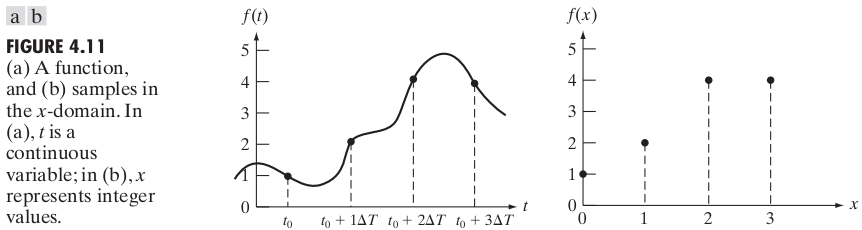
\includegraphics[width=\textwidth]{fig-4-11}
\end{figure}
\end{frame}

%----------------------------------------------------------------------------------------

\section{Extension to functions of 2 variables}

%----------------------------------------------------------------------------------------

\subsection{The 2-D impulse and its sifting property}

%----------------------------------------------------------------------------------------

\begin{frame}
\frametitle{The 2-D impulse}
The impulse $\delta(t,z)$ of continuous variables $t$ and $z$ is defined as
\begin{equation}
\delta(t,z) = \left \{
\begin{split}
\infty & \qquad \text{if}\ t=z=0\\
0 &  \qquad \text{otherwise}
\end{split}
\right .
\end{equation}
and
\begin{equation}
\int_{-\infty}^{\infty} \int_{-\infty}^{\infty} \delta(t,z) dt dz = 1.
\end{equation}
The sifting property of the 2-D impulse:
\begin{equation}
\int_{-\infty}^{\infty} \int_{-\infty}^{\infty} f(t,z) \delta(t-t_{0},z-z_{0}) dt dz = f(t_{0},z_{0}).
\end{equation}
\end{frame}

%----------------------------------------------------------------------------------------

\begin{frame}
The 2-D impulse for discrete variables $x$ and $y$ is defined as
\begin{equation}
\delta(x,y) = \left \{
\begin{split}
1 & \qquad \text{if}\ x=y=0\\
0 &  \qquad \text{otherwise}
\end{split}
\right .
\end{equation}
It sifting property:
\begin{equation}
\sum_{x=-\infty}^{\infty} \sum_{y=-\infty}^{\infty} f(x,y)\delta(x - x_{0},y - y_{0}) = f(x_{0},y_{0}).
\end{equation}
\begin{figure}
\centering
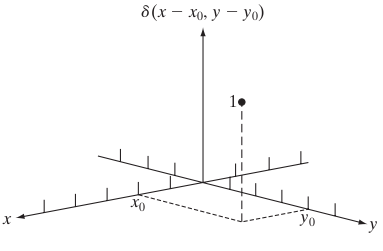
\includegraphics[width=.5\textwidth]{fig-4-12}
\end{figure}
\end{frame}

%----------------------------------------------------------------------------------------

\subsection{The 2-D continuous Fourier Transform pair}

%----------------------------------------------------------------------------------------

\begin{frame}
\frametitle{The 2-D continuous Fourier Transform pair}
Let $f(t,z)$ be a continuous function of two continuous variables $t$ and $z$.\\
The two dimensional Fourier transform pair is given by
\begin{equation}
F(\mu, \nu) = \int_{-\infty}^{\infty} \int_{-\infty}^{\infty} f(t,z) e^{-j2\pi (\mu t + \nu z)} dtdz,
\end{equation}
and
\begin{equation}
f(t,z) = \int_{-\infty}^{\infty} \int_{-\infty}^{\infty} F(\mu, \nu) e^{j2\pi (\mu t + \nu z	)} d\mu d\nu.
\end{equation}
Where $\mu$ and $\nu$ are the frequency variables.
\end{frame}

%----------------------------------------------------------------------------------------

\begin{frame}
\frametitle{Example}
\begin{figure}
\centering
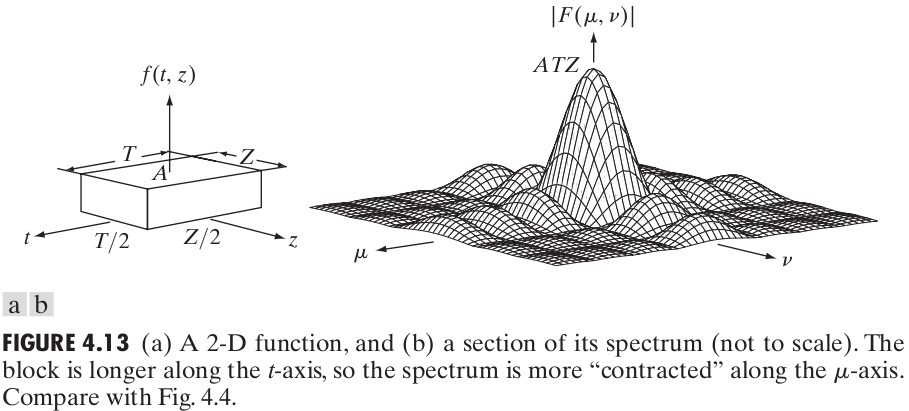
\includegraphics[width=.5\textwidth]{fig-4-13}
\end{figure}
\begin{figure}
\centering
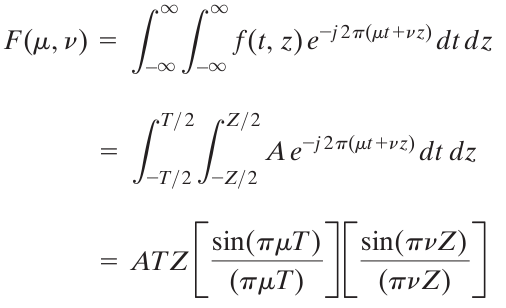
\includegraphics[width=.5\textwidth]{ex-4-5}
\end{figure}
\end{frame}

%----------------------------------------------------------------------------------------

\subsection{Two dimensional sampling and the 2-D sampling theorem}

%----------------------------------------------------------------------------------------

\begin{frame}
Sampling function (2-D impulse train):
\begin{equation}
s_{\Delta T \Delta Z} \sum_{m=-\infty}^{\infty} \sum_{n=-\infty}^{\infty} \delta(t-m\Delta T, z - n\Delta z).
\end{equation}
where $\Delta T$ and $\Delta z$ are the separations between samples in $t$- and $z$- axis of function $f(t,z)$.
\begin{figure}
\centering
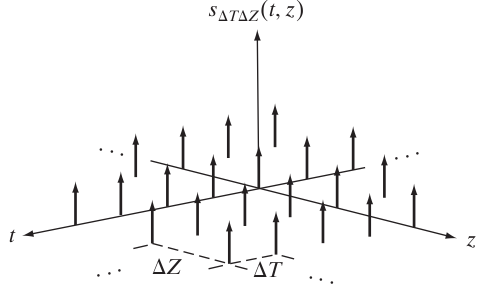
\includegraphics[width=.6\textwidth]{fig-4-14}
\end{figure}
\end{frame}

%----------------------------------------------------------------------------------------

\begin{frame}
\begin{itemize}
\item $f(t,z)$ is band-limited if $F(\mu,\nu) = 0$ for $|\mu| \leq \mu_{max}$ and $|\nu| \leq \nu_{max}$.
\end{itemize}
\begin{block}{\textit{Two-dimensional sampling theorem}}
A continuous, band-limited function $f(t,z)$ can be recovered with no error from a set of its samples if the sampling intervals are
\begin{equation}
\Delta T < \dfrac{1}{2\mu_{max}},
\end{equation}
and
\begin{equation}
\Delta Z < \dfrac{1}{2\nu_{max}}.
\end{equation}
\end{block}
\end{frame}

%----------------------------------------------------------------------------------------

\begin{frame}
No information is lost if a 2-D, band-limited continuous function is represented by samples acquired at rates greater than twice the highest frequency content of the function in both $\mu$- and $\nu$- directions.
\begin{figure}
\centering
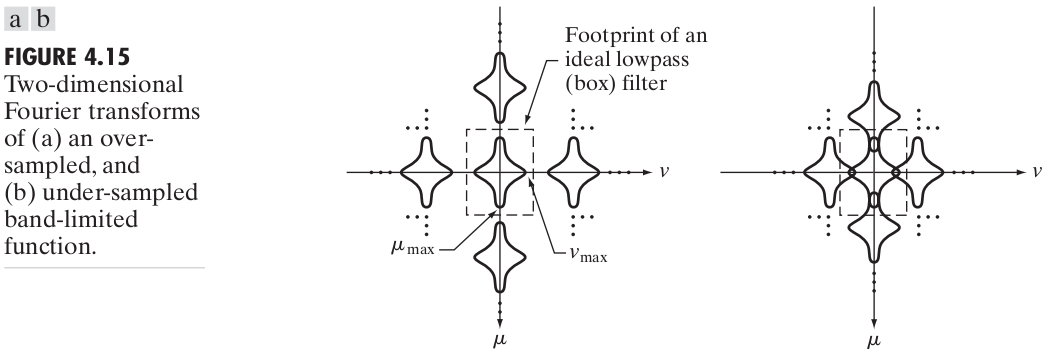
\includegraphics[width=\textwidth]{fig-4-15}
\end{figure}
\end{frame}

%----------------------------------------------------------------------------------------

\subsection{Aliasing in images}

%----------------------------------------------------------------------------------------

\subsubsection{Extension from 1-D aliasing}

%----------------------------------------------------------------------------------------

\begin{frame}
\frametitle{Aliasing in images}
We've seen that:
\begin{itemize}
\item Limiting the function's duration introduces corrupting
frequency components extending to infinity in the frequency domain.
\end{itemize}
\begin{block}{Image aliasing}
Two principal manifestations of aliasing in images;
\begin{itemize}
\item spatial (under sampling), and;
\item temporal (wagon wheel).
\end{itemize}
\end{block}
\end{frame}

%----------------------------------------------------------------------------------------

\begin{frame}
\frametitle{Spatial aliasing}
\begin{itemize}
\item Jagged\footnote{Denteado, chanfrado} lines.
\item Spurious highlights.
\item Appearance of frequency patterns.
\end{itemize}
\end{frame}

%----------------------------------------------------------------------------------------

\begin{frame}
\frametitle{Example}
\begin{itemize}
\item Consider a $96\times 96$ sensor.
\item Use it to digitize checkerboard patterns.
\end{itemize}
\begin{figure}
\centering
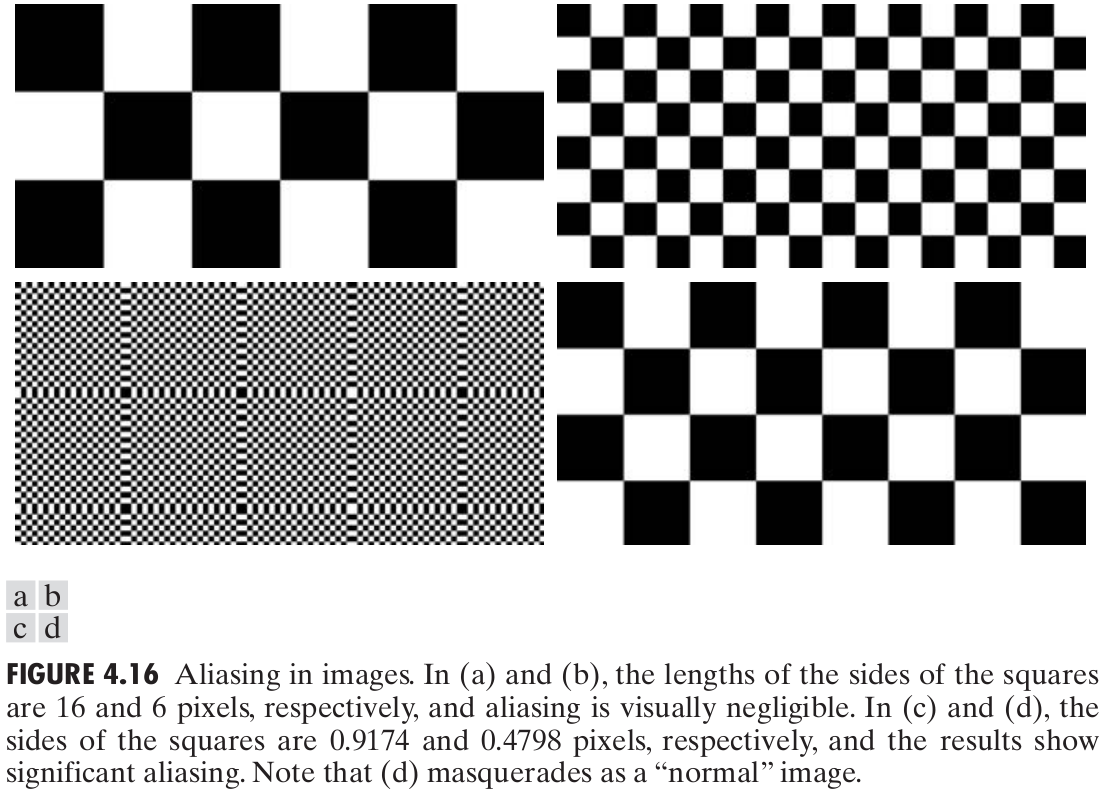
\includegraphics[width=.7\textwidth]{fig-4-16}
\end{figure}
\end{frame}

%----------------------------------------------------------------------------------------

\begin{frame}
Remember:
\begin{itemize}
\item Anti-aliasing must be done at the \textit{front-end}, i. e., before sampling occurs.
\end{itemize}
\end{frame}

%----------------------------------------------------------------------------------------

\subsection{2-D Discrete Fourier Transform (DFT)}

%----------------------------------------------------------------------------------------

\begin{frame}
\frametitle{2-D Discrete Fourier Transform (DFT)}
\end{frame}

%----------------------------------------------------------------------------------------

\section{Fourier Transform Properties}

%----------------------------------------------------------------------------------------

\begin{frame}
\frametitle{Fourier Transform Properties}
\end{frame}

%----------------------------------------------------------------------------------------

\section{Filtering in the Frequency Domain}

%----------------------------------------------------------------------------------------

\begin{frame}
\frametitle{Filtering in the Frequency Domain}
\end{frame}

%----------------------------------------------------------------------------------------

\section{Fast Fourier Transform (FFT)}

%----------------------------------------------------------------------------------------

\begin{frame}
\frametitle{Fast Fourier Transform}
\end{frame}

%----------------------------------------------------------------------------------------

\end{document}

%----------------------------------------------------------------------------------------
